\documentclass{article}
\usepackage{graphicx}
\usepackage{pdflscape}
\usepackage{lmodern}
\usepackage[T1]{fontenc}
\usepackage{textcomp}
\usepackage{underscore}
\graphicspath{./}

\newcommand{\schema}[2]{#1 (#2)}
\newcommand{\pkey}[1]{\underline{#1}}
\newcommand{\trightarrow}{\(\rightarrow\)}

\title{COMP3005 Project Design Document}
\author{Steven Pham}

\begin{document}
\maketitle
\section{ER Diagram}
The ER diagram is shown on the next page in landscape format.

\begin{landscape}
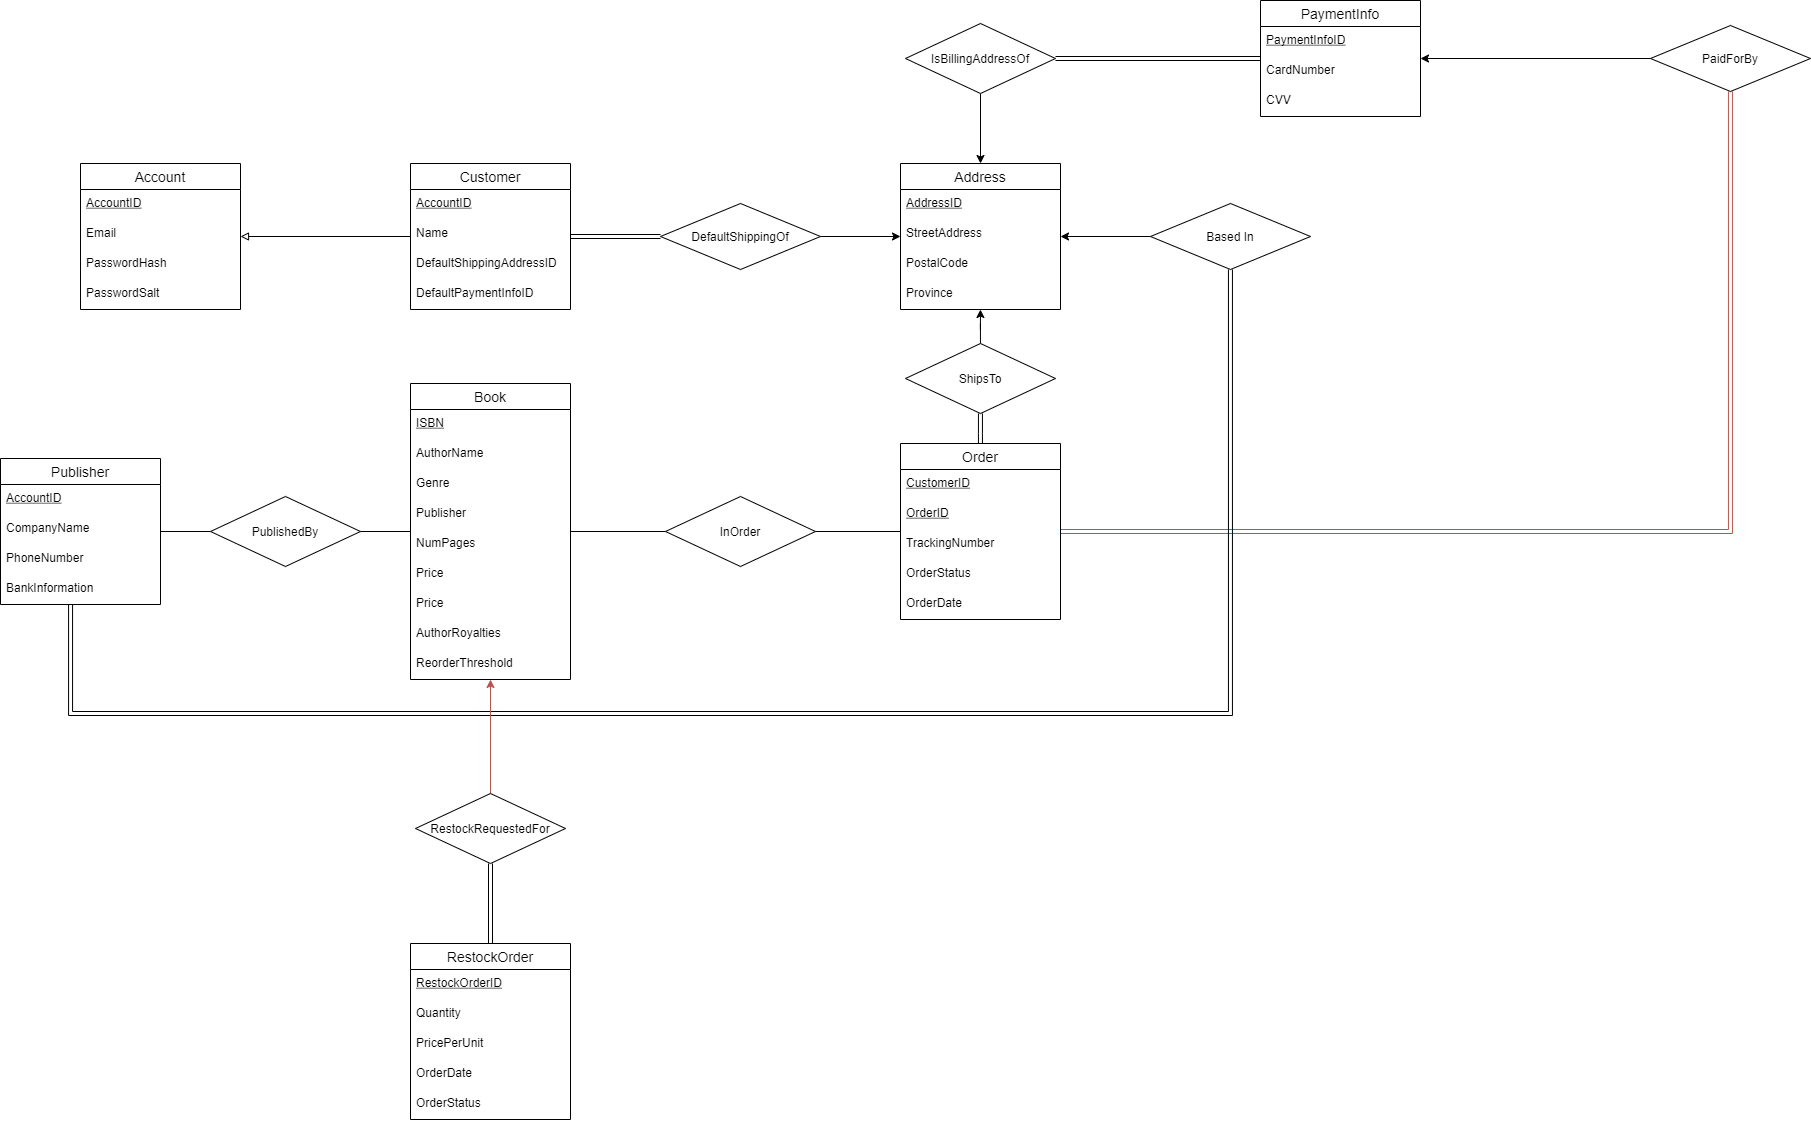
\includegraphics[width=\textwidth]{er}
\end{landscape}

\section{Relations Schema}
The above ER diagram can be broken down into the relation schema below.
\begin{itemize}
        \item \schema{book}{\pkey{isbn}, author_name, genre, publisher, num_pages}
\end{itemize}

\section{Functional Dependencies}
\begin{itemize}
  \item BookISBN \(\rightarrow\) AuthorName, Genre, Publisher, NumPages, Price
  \item CustomerID \(\rightarrow\) CustomerName, CustomerEmail, PassHash, PassSalt, DefaultShippingAddressID, DefaultPaymentInfoID
  \item PaymentInfoID \(\rightarrow\) CardNumber, CVV, BillingAddressID
  \item AddressID \(\rightarrow\) StreetAddress, PostalCode, Province
  \item OrderID \(\rightarrow\) CustomerID, ShippingAddressID, PaymentInfoID, OrderStatus, OrderTrackingNum
  \item OrderID, BookISBN \(\rightarrow\) OrderQuantity
  \item CustomerID, BookISBN \(\rightarrow\) CartQuantity
\end{itemize}
\end{document}
